\subsection{Common-gap selection and independent evaluation}
The two-arm experiment uses the designs in Section~\ref{sec:experiment-random}.
Each conditional cell fixes $T,H,\Delta$ and the sign before drawing
rewards. If $n_0=T-H$, the sole anchor's sufficient statistics at the
first competitor arrival are $(N_0,S_0)=(n_0,\operatorname{Bin}(n_0,1/2))$.
This compression has exactly the same law as the full forced prefix.
MC-MOSS uses these statistics and a local clock starting at one;
Fresh-H MOSS discards them and uses the fixed remaining horizon $H$.
Both indices have the form
$\widehat\mu_i+\sqrt{[\log\{u/(2N_i)\}]_+/N_i}$,
with $u=s$ at the $s$th post-arrival decision for MC-MOSS and $u=H$
for Fresh-H MOSS. Unobserved arms have infinite index, and ties favor
the anchor. A shared independent uniform variate at each decision
couples the two methods' rewards within a replication.

Development and held-out strata use 64 and 128 replications. The seed
of stratum $(m,j,e)$ is
$2026101303+o+100000m+1000j+e$, where $e$ indexes the gap/sign grid
and $o=0$ for development and $o=10000000$ for evaluation.
All seeds in these two sets are distinct. For each method and arrival
law, development means select either one common grid member or one
member for every $H$. Only the former defines a lawful reward
environment fixed before the random schedule. The latter is a
schedule-dependent benchmark. Different methods may select different
environments, so their displayed selected risks are not a paired
comparison under one common environment.

For selected stratum losses $R_{jr}$ and known probabilities $p_j$, the
reported estimate and standard error are
\[
 \widehat r=\sum_jp_j\overline R_j,\qquad
 \widehat{\operatorname{se}}(\widehat r)
 =\left\{\sum_jp_j^2s_j^2/128\right\}^{1/2},
\]
where $s_j^2$ is the unbiased sample variance. Independent strata
justify this expression. Conditional on the development selections,
these are unbiased estimates of the selected environments' risks.
They are not unbiased estimates of a maximum over the grid.

The additional direct-draw experiment samples 2048 lifetimes from each
arrival law, keeps its development-selected common environment fixed,
and generates new rewards. It has its own random stream. Its ordinary
Monte Carlo standard error includes both arrival and reward variation.
The two estimates in Table~\ref{tab:random-selected} therefore need not
coincide. All endpoints, selected indices, gap values, signs and seeds
are saved in the released CSV and compressed raw arrays.

\begin{table}[tb]
\centering\small
\caption{Selected-environment risks at $T=16384$. Parentheses are
Monte Carlo standard errors. ``Specific'' permits the development
environment to depend on the realized schedule. ``Direct common''
uses 2048 new random schedules under the common environment.}
\label{tab:random-selected}
\begin{tabular}{llrrr}\toprule
Arrival law & Policy & Common & Specific & Direct common\\\midrule
Inverse square root & Fresh-H & 1.321 (0.018) & 1.977 (0.026) & 1.319 (0.053) \\
Inverse square root & MC & 1.384 (0.000) & 1.781 (0.020) & 1.302 (0.035) \\
Uniform scales & Fresh-H & 13.339 (0.440) & 14.768 (0.399) & 12.139 (0.529) \\
Uniform scales & MC & 11.262 (0.366) & 13.459 (0.398) & 11.377 (0.458) \\
Short concentrated & Fresh-H & 0.675 (0.006) & 0.738 (0.005) & 0.667 (0.014) \\
Short concentrated & MC & 0.721 (0.000) & 0.731 (0.002) & 0.711 (0.014) \\
Two longest scales & Fresh-H & 47.389 (1.753) & 43.332 (1.546) & 45.121 (0.698) \\
Two longest scales & MC & 41.920 (1.420) & 40.544 (1.554) & 39.202 (0.648) \\
Longest scale & Fresh-H & 57.365 (2.771) & 57.365 (2.771) & 60.868 (0.717) \\
Longest scale & MC & 57.818 (2.921) & 57.818 (2.921) & 57.591 (0.742) \\
\bottomrule\end{tabular}
\end{table}

\begin{figure}[p]\centering
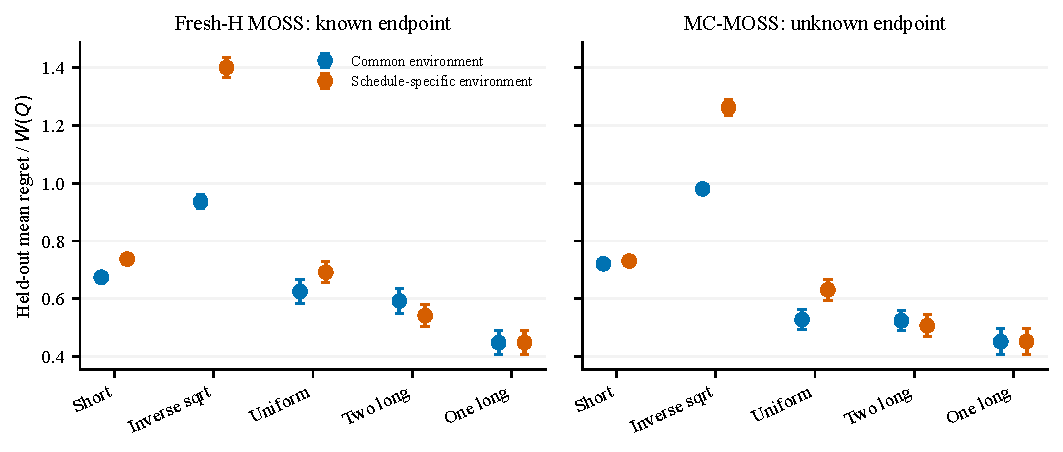
\includegraphics[width=\linewidth]{figures_v2/random_mixture_comparison.pdf}
\caption{Held-out common and schedule-specific selected risks at
$T=16384$ for all five arrival laws, divided by $W(Q)$. Bars are
$1.96$ stratified Monte Carlo standard errors. Selection takes place
on an independent finite development sample, so the held-out
ordering need not agree with the order of exact grid maxima.}
\label{fig:random-mixtures}
\end{figure}

The full study executes 451,072 policy trajectories and 687,147,832
post-arrival policy decisions, including development, held-out and
direct-draw runs. The zero-regret forced prefixes are compressed as
described above. Independent verification replays 1,008 conditional
trajectories and reconstructs all 2,992 grid summaries and all 80
selected held-out summaries from the raw arrays.

\subsection{The two-batch stretch implementation}
Section~\ref{sec:stretch-experiment} specifies the fixed template and
common mean vectors. Before the first batch, the count is $T-4H$ and
the anchor's success count is drawn from $\operatorname{Bin}(T-4H,1/2)$.
At the first arrival, the informed rule infers $H$ from $T$ and the
observed time and runs fresh MOSS for $3H$ rounds on three arms.
At the second arrival it runs fresh MOSS for $H$ rounds on five arms.
MC-MOSS retains all prefix and intermediate observations. Every loss
after the first batch is recorded, including the complete $3H$ prefix
before the final batch.

The development and held-out base seeds are 841013 and 951013; the
stratum seed adds $100000m+1000j+r$. The sets are disjoint over the
simulated indices. Both methods and all grid members share the reward
uniforms for a fixed stratum and replication. Development selects one
environment for each $(m,Q)$ using the informed rule's risk. Both rules
then face that same environment at every stretch in evaluation.
Unlike Table~\ref{tab:random-selected}, this is a common-environment
comparison across methods; it does not separately maximize MC-MOSS's
risk over the grid.

The 84,480 stratum trajectories require 111,390,720 post-first-arrival
policy decisions. Nine full-calendar comparisons verify the prefix
compression against the original MC implementation. The saved-data
audit checks every interval-loss decomposition, all 12 development
selections and all 24 held-out summaries. Complexity curves are
computed independently of rewards; the capacity calculation agrees
with $2\sqrt{3H/2}+2\min\{H/2,\sqrt{H/2}\}$.
